\section{Results and Discussion}
\label{sec:results}

\subsection{Core Finding: The Planning-Execution Gap is Measurable and Structural}

The analysis begins with a fundamental question: when accurate forecasts and operational feasibility diverge, how often does this matter? The answer is striking: in 91.1\% of evaluation groups, the strategy that minimizes WAPE is NOT the strategy that minimizes operational planning loss, and this is structural across datasets, run modes, and execution-risk scenarios, not a marginal effect. Accuracy-first strategies have a PEG rate of 15.4\% of periods (execution violations exceeding operational capacity), compared with 2.7\% for the best deployable operational-loss strategy---a 12.7-percentage-point gap. For a typical 365-period planning year, that difference means accuracy-first strategies require emergency execution handling roughly 56 times versus 10 times for operationally optimized strategies: the planning-execution gap is measurable, quantifiable, and operationally consequential.

When accuracy-best and deployment-best strategies diverge, no single method is universally optimal; different strategy families serve different operational constraints, starting with ensemble methods.

\subsection{Finding 1: Ensemble Methods Provide Low-Disruption First Rollout}

Ensemble averaging combines candidate forecasts into one blended prediction---if Model A predicts 100 units and Model B predicts 120, the ensemble predicts 110---which dampens abrupt plan movement while retaining both models' information. In the Favorita evidence, Global Best (accuracy-first) reaches WAPE 17.7\% with execution violation rate 42.1\% (normalized loss 1.550), while Simple Ensemble reaches WAPE 17.4\% with violation rate 5.2\% (normalized loss 1.422): a 36.9pp violation reduction at no WAPE cost. Ensemble is therefore a practical first-rollout candidate wherever plan movement is costly and requires no new model validation or monitoring infrastructure, though it offers little advantage where WAPE accuracy is itself the competitive edge (e.g., predictable, high-value, low-volume demand).

Figure~\ref{fig:frontier} places all nine baseline-scenario strategies on the same accuracy-execution plane. WAPE and execution penalty do not move together: Global Best and Family Best sit almost on top of each other in the upper-middle region, while Simple Ensemble and the smoothing-based strategies reach comparable or better WAPE at a fraction of the execution penalty. The Realized-Demand Oracle---the non-deployable reference that tracks realized demand exactly---has zero forecast error but the single highest execution penalty in the panel: the ``curse of accuracy'' introduced in Section~\ref{sec:methods}, where perfect demand tracking moves the plan faster than operations can absorb.

\begin{figure}[H]
\centering
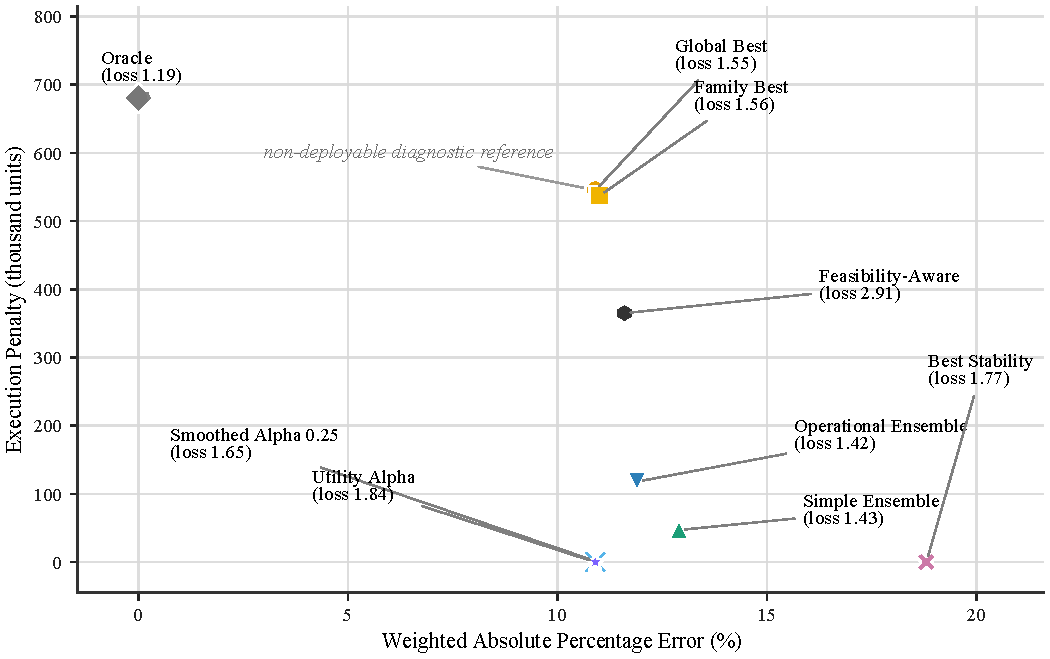
\includegraphics[width=0.67\linewidth]{figures/favorita_accuracy_execution_frontier.pdf}
\caption{Favorita accuracy-execution frontier, baseline scenario: WAPE versus execution penalty for all nine deployable strategies plus the non-deployable Oracle reference, each labeled with its normalized planning loss.}
\label{fig:frontier}
\end{figure}

\subsection{Finding 2: Smoothing and DP Serve Different Governance Regimes}

When ensemble's improvement is insufficient, smoothing and dynamic programming cover the remaining operational constraints. \textbf{Smoothing} slows adaptation by blending the new plan with the previous period's, trading response speed for stability: Best Stability ($\alpha \approx 0.25$) reaches WAPE 20.6\% with execution violation rate 0.03\% (normalized loss 1.220)---a 2.9pp WAPE cost for 99.97\% execution stability. It is worth this cost only where execution capacity is so constrained that plan stability outweighs accuracy, e.g., single-source suppliers or systems already at maximum utilization.

\textbf{Dynamic programming} accounts for future switching costs that one-period greedy selection ignores: staying with an already-approved model can beat switching to a marginally better one once tomorrow's approval cost is counted. The greedy-to-DP gap (0.044, small when switching cost is low) and DP-oracle gap (0.198) quantify this myopia and the feasibility remaining after DP selection; DP is worth its complexity when changes require multi-step approval or system coordination, and budgeted DP adds a hard annual switching limit under strict change-control governance.

\subsection{Finding 3: Planning Hierarchy Changes Optimal Strategy}

The most striking finding is that different aggregation levels favor fundamentally different strategies, challenging the ``one global forecasting model'' paradigm. In M5, the finest grain (item-store, sparse and volatile) favors Smoothed Alpha 0.25 (WAPE 25.4\%, violation 0.0\%, loss 1.026) because smoothing dampens noise without model changes; aggregating to department-store demand shifts the advantage to Operational Ensemble (WAPE 15.9\%, violation 12.9\%, loss 0.991), and category-store aggregation keeps it (WAPE 14.9\%, violation 9.6\%, loss 1.033), since ensembles can now capture different models' information once demand is stable. Supply chains should therefore not deploy one global model across all planning grains: item-level favors smoothing, department- and category-level favor ensemble, with DP added where governance matters---planning-system architecture should be hierarchy-aware for exactly this reason.

\subsection{Model-Rollout Protocol: From Evidence to Practice}
\label{sec:protocol}

Findings 1--3 above are diagnostic: they explain \emph{why} strategies diverge. This section turns that diagnosis into the paper's primary practical deliverable---a five-step protocol that a planning team can follow to go from a set of candidate forecasts to a specific, defensible deployment decision.

\begin{figure}[H]
\centering
\resizebox{\linewidth}{!}{% Model-Rollout Protocol: the paper's primary practical deliverable.
% Included via \input in sections/05_results_discussion.tex (Figure 3).
% No formulas here by design -- all equations live in the body text (Section 3);
% this figure's job is to make the decision architecture readable at a glance.
\begin{tikzpicture}[
  font=\sffamily,
  >=Latex,
  every node/.style={align=center},
  stepbox/.style={draw=black!70, fill=gray!8, rounded corners=2pt, minimum height=0.85cm, minimum width=3.55cm, font=\sffamily\footnotesize, inner sep=2pt},
  step5box/.style={draw=teal!80!black, thick, fill=teal!8, rounded corners=3pt, minimum height=0.85cm, font=\sffamily\bfseries\small},
  lanehdr/.style={draw=none, fill=none, font=\sffamily\bfseries\footnotesize},
  branchlbl/.style={draw=black!45, fill=white, rounded corners=1.5pt, minimum height=0.42cm, minimum width=2.3cm, font=\sffamily\footnotesize, inner sep=1pt},
  leafbox/.style={rounded corners=1.5pt, minimum height=0.62cm, minimum width=2.45cm, font=\sffamily\footnotesize, inner sep=2pt, thick},
  note/.style={font=\sffamily\itshape\scriptsize, text=black!60},
]

% ===== Steps 1-4 pipeline =====
\node[stepbox] (st1) at (2.0,10.6) {\textbf{1. Screen by Accuracy}\\ \normalfont Remove WAPE outliers};
\node[stepbox] (st2) at (6.0,10.6) {\textbf{2. Convert to Signals}\\ \normalfont Forecast $\to$ inventory target};
\node[stepbox] (st3) at (10.0,10.6) {\textbf{3. Measure Feasibility}\\ \normalfont PEG rate, planning loss};
\node[stepbox] (st4) at (14.0,10.6) {\textbf{4. Stress-Test Scenarios}\\ \normalfont Low $\to$ severe execution risk};

\draw[->, black!70] (st1.east) -- (st2.west);
\draw[->, black!70] (st2.east) -- (st3.west);
\draw[->, black!70] (st3.east) -- (st4.west);

% ===== Step 5 header =====
\node[step5box, minimum width=15.3cm] (st5) at (8.0,9.2) {\textbf{5. Select by Operating Condition} --- three independent operational readings, evaluated together};
\foreach \s in {st1,st2,st3,st4} {
  \draw[->, black!70] (\s.south) -- ++(0,-0.35) -| (st5.north);
}

% ===== Three decision lanes =====
% Lane A: Execution Flexibility (blue)
\node[lanehdr, text=blue!55!black] (hA) at (2.6,8.15) {Execution Flexibility};
\node[branchlbl] (aFlex) at (1.3,7.25) {Flexible};
\node[branchlbl] (aCon)  at (4.0,7.25) {Constrained};
\node[leafbox, draw=blue!55, fill=blue!6] (aLeaf1) at (1.3,6.15) {Accuracy-First\\ or Ensemble};
\node[leafbox, draw=blue!55, fill=blue!6] (aLeaf2) at (4.0,6.15) {Ensemble\\ or Smoothing};

% Lane B: Governance Maturity (violet)
\node[lanehdr, text=violet!55!black] (hB) at (8.0,8.15) {Governance Maturity};
\node[branchlbl] (bHigh) at (6.7,7.25) {High};
\node[branchlbl] (bLow)  at (9.4,7.25) {Low};
\node[leafbox, draw=violet!55, fill=violet!6] (bLeaf1) at (6.7,6.15) {DP or\\ Budgeted DP};
\node[leafbox, draw=violet!55, fill=violet!6] (bLeaf2) at (9.4,6.15) {Simpler policy\\ (Ensemble)};

% Lane C: Planning Hierarchy (teal-green)
\node[lanehdr, text=teal!60!black] (hC) at (13.4,8.15) {Planning Hierarchy};
\node[branchlbl] (cItem) at (12.1,7.25) {Item-level};
\node[branchlbl] (cAgg)  at (14.8,7.25) {Dept./Category};
\node[leafbox, draw=teal!60, fill=teal!6] (cLeaf1) at (12.1,6.15) {Smoothing-\\ leaning};
\node[leafbox, draw=teal!60, fill=teal!6] (cLeaf2) at (14.8,6.15) {Ensemble-\\ leaning};

\draw[->, black!70] (st5.220) -- ++(0,-0.3) -| (hA.north);
\draw[->, black!70] (st5.south) -- ++(0,-0.3) -| (hB.north);
\draw[->, black!70] (st5.-40) -- ++(0,-0.3) -| (hC.north);

\draw[->, black!70] (hA.south) -- ++(0,-0.18) -| (aFlex.north);
\draw[->, black!70] (hA.south) -- ++(0,-0.18) -| (aCon.north);
\draw[->, black!70] (aFlex.south) -- (aLeaf1.north);
\draw[->, black!70] (aCon.south) -- (aLeaf2.north);

\draw[->, black!70] (hB.south) -- ++(0,-0.18) -| (bHigh.north);
\draw[->, black!70] (hB.south) -- ++(0,-0.18) -| (bLow.north);
\draw[->, black!70] (bHigh.south) -- (bLeaf1.north);
\draw[->, black!70] (bLow.south) -- (bLeaf2.north);

\draw[->, black!70] (hC.south) -- ++(0,-0.18) -| (cItem.north);
\draw[->, black!70] (hC.south) -- ++(0,-0.18) -| (cAgg.north);
\draw[->, black!70] (cItem.south) -- (cLeaf1.north);
\draw[->, black!70] (cAgg.south) -- (cLeaf2.north);

% ===== Bottom note =====
\node[note] at (8.0,5.15) {Read the three lanes independently, then prioritize the most operationally binding constraint---e.g.,\\ a hard governance ceiling overrides an accuracy preference (Table~\ref{tab:deployment-guidance} lists the full mapping).};

\end{tikzpicture}
}
\caption{Model-rollout protocol, the paper's primary practical output: Steps 1--4 screen and score every candidate, and Step 5 combines three operational lanes---execution flexibility, governance maturity, planning hierarchy---into a strategy recommendation.}
\label{fig:protocol}
\end{figure}

Steps 1--4, shown across the top of Figure~\ref{fig:protocol}, are a short mechanical pipeline: screen out clearly weak forecasts (WAPE $>$ 30\%), convert each survivor into an inventory target using organization-specific policies, measure its PEG rate and normalized planning loss, and stress-test it across execution-risk scenarios from low to severe. Step 5 is the decision core, combining three operational readings that were each established by a Finding above: execution flexibility (Finding 1) points toward accuracy-first or ensemble when flexible, ensemble or smoothing when constrained; governance maturity (Finding 2) points toward DP or budgeted DP when switching approval is costly, simpler policies otherwise; and planning hierarchy (Finding 3) points toward smoothing at fine grain, ensemble at coarser grain. Table~\ref{tab:deployment-guidance} gives the complete condition-to-policy mapping behind each leaf.

\begin{table}[htbp]
\centering
\caption{Deployment strategy families and rollout conditions.}
\label{tab:deployment-guidance}
\scriptsize
\begin{tabular}{@{}p{0.29\linewidth}p{0.30\linewidth}p{0.31\linewidth}@{}}
\toprule
\textbf{Operating condition} & \textbf{Recommended deployment policy} & \textbf{Reason} \\
\midrule
Flexible execution capacity & Accuracy-first or ensemble & WAPE gains can be useful when plan movement is absorbable, but feasibility screening remains required. \\
Moderate execution constraint & Ensemble & Averaging can dampen model-specific swings while retaining adaptation. \\
Severe execution constraint & Smoothing & Gradual adaptation can reduce execution burden when abrupt plan movement is costly. \\
High switching governance & DP or budgeted DP & Horizon-aware selection accounts for future switching and coordination burden. \\
Multi-level hierarchy & Choose by planning grain & Item, department, and category planning can favor different deployment mechanisms. \\
\bottomrule
\end{tabular}
\end{table}


The protocol is structured evaluation, not single-method prescription: it provides a repeatable procedure, not a universal answer, and the final decision still depends on organizational constraints and risk tolerance. Section~\ref{sec:validation} tests whether this procedure holds up outside the conditions it was built on.

\subsection{Robustness and Validation}
\label{sec:validation}

Four complementary checks confirm that findings are structural, not data artifacts, and that the protocol in Section~\ref{sec:protocol} is trustworthy outside the conditions it was built on.

\subsubsection{Baseline and External Validation: Is This a Real Problem?}

The 91.1\% mismatch rate and 12.7pp PEG-rate gap demonstrate that WAPE-best selection and deployment-best selection answer fundamentally different questions; the study does not claim feasibility-aware strategies always dominate, only that the operational deployment criterion is measurably distinct from the accuracy criterion. This divergence is not unique to the present data---it replicates a pattern already established in the predict-then-optimize literature, where Elmachtoub and Grigas (2022) show that prediction-loss-minimizing models are not necessarily loss-minimizing for the downstream decision, and Jia et al. (2025) report the same divergence for inventory-routing decisions. This paper's contribution is not the divergence itself but a feasibility-specific metric (PEG rate) and an evaluation layer that makes it measurable for demand planning specifically, where prior work has largely addressed routing and pricing decisions instead.

\subsubsection{Scenario Validation: Does Execution Pressure Change Rankings?}

DataCo-informed execution-risk scenarios validate whether tighter execution constraints change strategy rankings: as execution-risk weights increase from low to severe, ensemble and smoothing methods become relatively more attractive than accuracy-first selection, supporting scenario testing as a deployment practice since the optimal model for a flexible environment may not be optimal for a constrained one.

Figure~\ref{fig:scenario-loss} orders the five scenarios by increasing severity and tracks all nine strategies through each; the y-axis is broken because Feasibility-Aware, an early naive selector, sits nearly twice as high as everyone else and would otherwise compress the eight competitive strategies into an unreadable band. Among those eight, Global Best and Family Best rise fastest as execution risk tightens (1.55 at baseline to 2.00 at severe), while Simple Ensemble, Operational Ensemble, and the smoothing-based strategies stay comparatively flat---direct visual evidence that accuracy-first selection is the strategy most exposed to execution-risk escalation.

\begin{figure}[H]
\centering

\includegraphics[width=0.67\linewidth]{figures/favorita_normalized_loss_by_execution_scenario.pdf}
\caption{Favorita normalized planning loss across execution-risk scenarios, ordered by increasing severity. The broken y-axis separates Feasibility-Aware (top panel) from the eight competitive strategies (bottom panel).}
\label{fig:scenario-loss}
\end{figure}

Algorithmic validation asks the complementary question of whether planning ahead has value: the greedy-to-DP gap (0.044) measures the cost of myopic one-period selection, small when simple policies are adequate and material when switching governance costs (approval workflows, system change cycles) make DP's planning-ahead value important---confirming DP is a deliberate choice for high-governance environments, not a universal improvement.

\subsubsection{Cross-Dataset Robustness Validation}

Favorita (daily granularity, rich context) is the main proof of concept; M5 (hierarchical, sparse demand) is re-evaluated under the same DataCo-calibrated severity scenarios as Favorita and extends the finding by showing that hierarchy and sparsity genuinely change the optimal strategy rather than adding noise; Walmart (weekly cadence, business context) confirms the same 80.0\% accuracy-first mismatch rate at a different temporal frequency, showing the gap is not limited to daily retail grocery planning. Together, the four checks support the thesis that feasibility-constrained planning is a multi-objective tradeoff surface, not a single-method leaderboard, and that each lane of the Section~\ref{sec:protocol} protocol rests on evidence rather than assumption: baseline validation establishes that the gap itself is real, scenario and algorithmic validation justify the execution-flexibility and governance-maturity lanes specifically, and cross-dataset validation justifies the planning-hierarchy lane. A planner who follows Figure~\ref{fig:protocol} is relying on a procedure stress-tested against the operational conditions it is meant to handle, not on advice tuned to a single dataset.

\subsection{Limitations and Future Work}

Public datasets do not observe the full internal cost of execution changes, planner overrides, or system reconfiguration, so execution capacity is proxied rather than directly measured; internal operational data could improve this calibration. The study also focuses on model-selection strategy rather than real-time plan adjustment or human planner intervention---extending the framework to planner workflows and collaborative replanning is a natural next step.

